\hypertarget{retour-aux-origines-uxe0-quuxe9bec}{%
\section{Retour aux origines à
Québec}\label{retour-aux-origines-uxe0-quuxe9bec}}

\emph{Lundi 22 octobre 2018}

Notre arrivée à Québec se fait au milieu d'une actualité brûlante : en
effet, le Canada a légalisé le \emph{pot}, c'est à dire le cannabis, et
cette légalisation entre en vigueur cette semaine. Un sujet de société
qui ne laisse personne indifférent, ce que l'on voit à la fois dans les
titres de journaux, les discussions de comptoirs et les longues files
d'attentes dans les nouvellement ouvertes officines du pot.

Mais Québec, c'est aussi un retour aux origines. Un retour aux origines
de la famille Le Bourdais. Une famille dont la localisation géographique
a fait une boucle. Un (seul ?) breton qui émigre au Canada, colonie
française. Des descendants canadiens. Dont certains émigrent aux
États-Unis pour chercher du travail. L'un d'entre-eux vient en France
lors de la première guerre mondiale, et s'y fixe. Et des années plus
tard, l'un des canadiens établit ce cheminement à travers le temps et
l'espace et croise la route d'un français. Les familles se découvrent.
Et me donnent l'occasion de décrire cette étonnante histoire dans ces
grandes lignes.

\begin{figure}
\centering
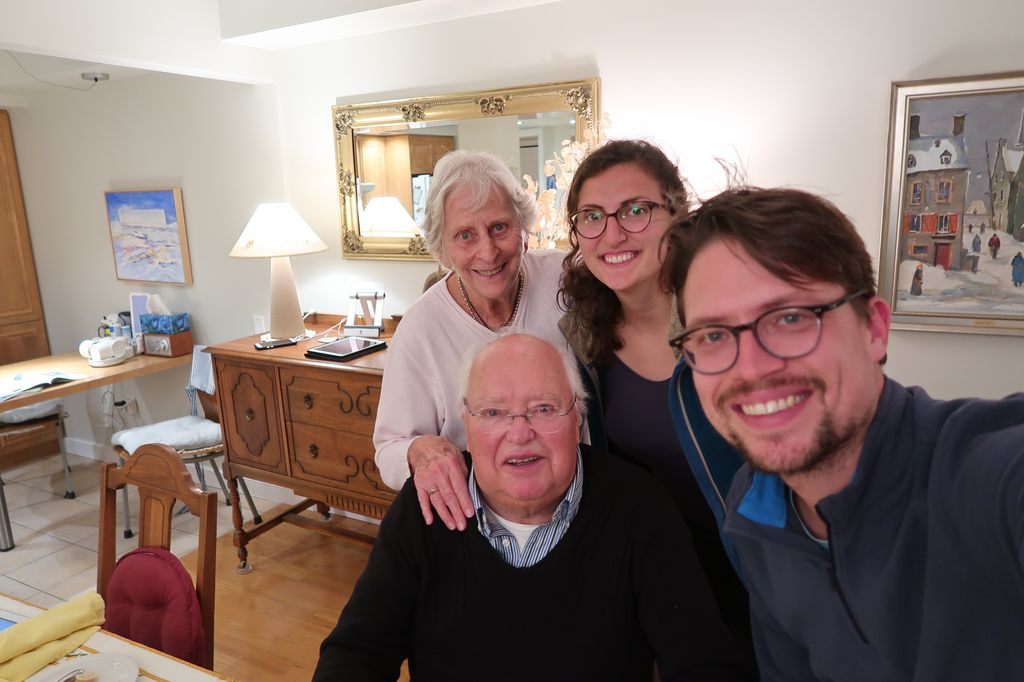
\includegraphics{images/20181022_GuySue.JPG}
\caption{Guy et Suzanne.}
\end{figure}

Finalement, c'est Guy Le Bourdais l'artisan principal, l'archéologue
pourrait-on dire, de cette ré-découverte. Lui et Suzanne nous on fait le
bonheur de nous emmener découvrir l'un des lieux de cette histoire,
l'Islet. On y trouve une maison des années 1800, et qui fait le trait
d'union entre les ancêtres de Guy et les miens.

\begin{figure}
\centering
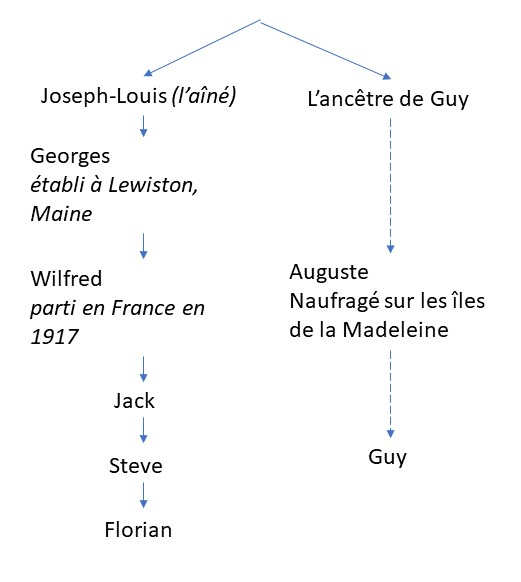
\includegraphics[width=0.5\textwidth]{images/20181022_arbre_genealogique.jpg}
\caption{L'arbre généalogique approximatif des dernières générations.}
\end{figure}

C'est aussi l'occasion de découvrir les oies, qui je ne connaissais
qu'en chanson grâce au \emph{Tour de l'île} de Félix Leclerc. Et elles
sont nombreuses, aux abords du grand fleuve !

\begin{quote}
Au mois de mai, à marée basse,

Voilà les oies, depuis des siècles

Au mois de juin, parties les oies,

Et nous les gens, les descendants de La Rochelle,

Présents tout le temps,

Surtout l'hiver, comme les arbres
\end{quote}

\begin{figure}
\centering
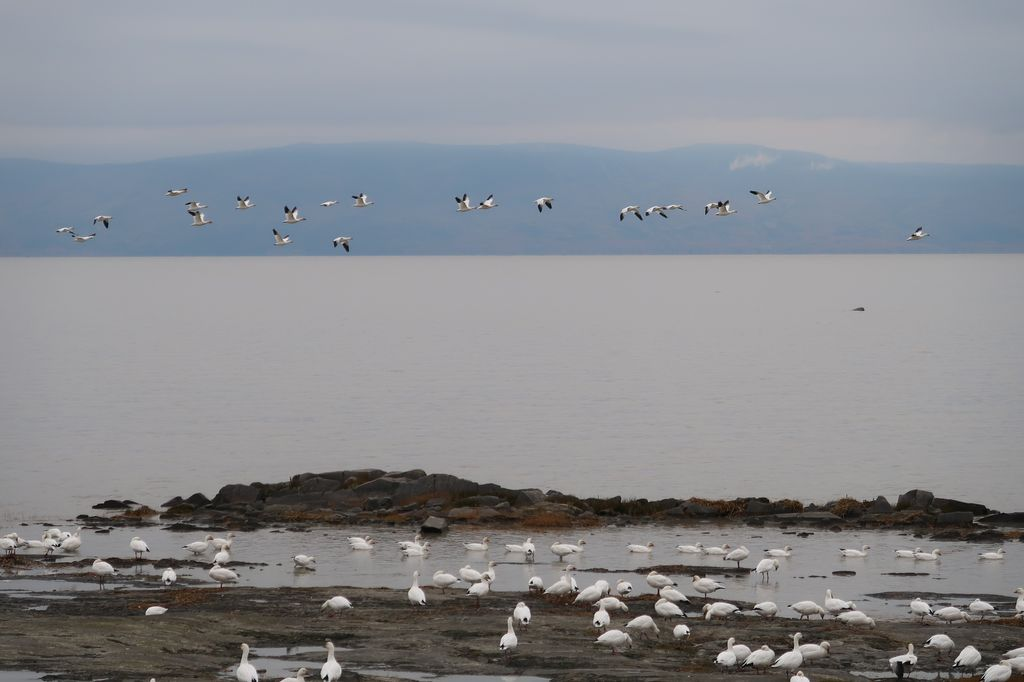
\includegraphics{images/20181022_oies.JPG}
\caption{Les oies, entre ciel et terre.}
\end{figure}

D'ailleurs, notre retour a été bien sûr l'occasion de faire un tour sur
cette fameuse île. Nous y avons trouvé les couleurs qui font la
réputation du Canada et le bonheur des photographes amateurs que nous
sommes. Le musée Felix Leclerc y garde la mémoire du grand chansonnier,
dont le parcours semble avoir été tout de même mouvementé. On y retrouve
même Suzanne, au sein d'un joli portrait qui voit le poète se voir
remettre une médaille du gouvernement du Québec. Quand je vois cette
photo, je ne peux pas m'empêcher de voir le lien entre la chanson, ma
famille et la volonté d'indépendance de nombre d'habitants de cette
région.

\begin{figure}
\centering
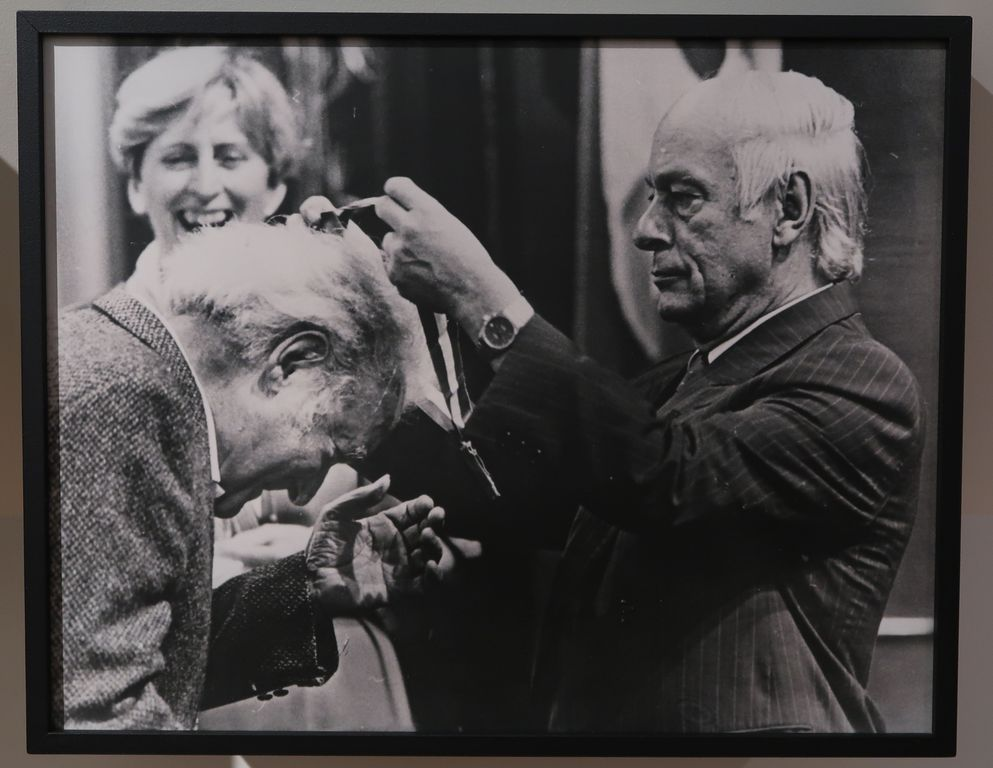
\includegraphics{images/20181022_FelixLeclerc.JPG}
\caption{Une photo en noir et blanc où l'on retrouve un premier
ministre, un artiste et... Suzanne !}
\end{figure}

Quelle chance d'avoir trouvé cette famille à l'autre bout de
l'Atlantique ! Je vous ai déjà parlé de Guy et Suzanne, dont la bonne
humeur et la curiosité reste vive, après un si long parcours. Mais il y
a aussi la famille d'Anne, Christian et Philippe. Philippe, qui nous
aura reçu avec tant de chansons exécutées de manière virtuose sur les
nombreuses guitares que compte la maison. Anne et Christian avec leur
hospitalité incomparable, qui fait qu'on se sent à la maison sans
l'ombre d'un doute. Et puis tous ces moments passés au son du doux
dialecte québecois.

Je vous laisse sur une anecdote qui pourrait vous resservir si jamais
vous avez la chance de visiter Québec. Savez-vous d'où vient le nom de
\emph{Québec} ?

Réponse :

\begin{figure}
\centering
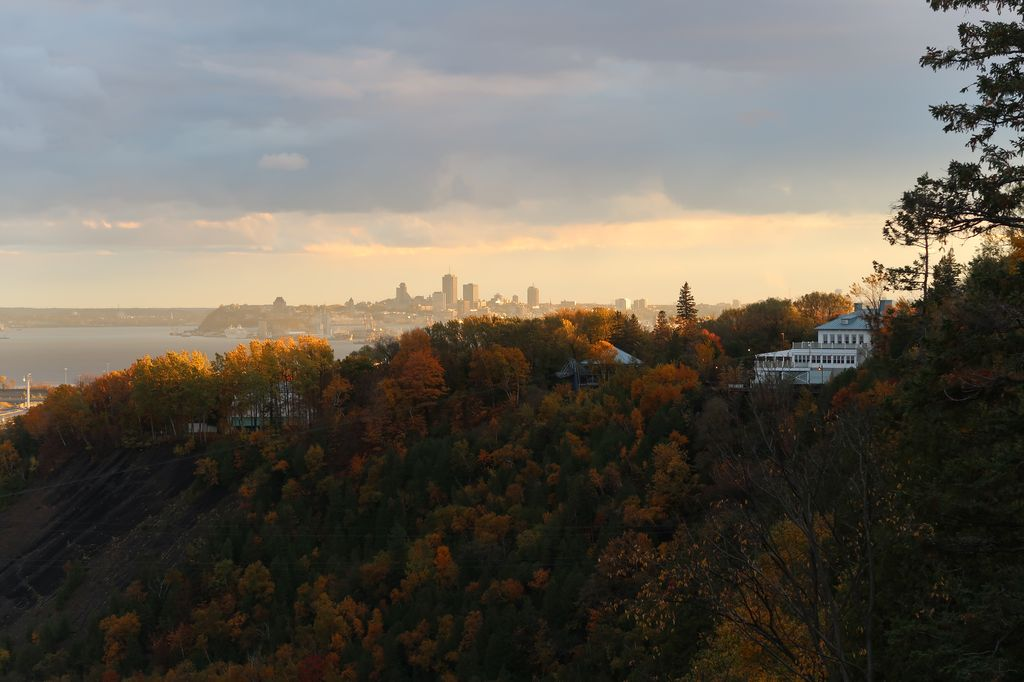
\includegraphics{images/20181022_quebec.JPG}
\caption{Québec : là où "le fleuve devient étroit" (vue depuis les
chutes de Montmorency).}
\end{figure}

\emph{Florian}
